\documentclass[a4paper,12pt]{article}
\usepackage{fullpage}
\usepackage{hyperref}
\usepackage{url}
\usepackage{amssymb}
\usepackage{graphicx}
%\usepackage{polski}
\usepackage[utf8]{inputenc}

\setlength{\parindent}{0pt}
\addtolength{\parskip}{\baselineskip}

\title{3rd Year Group Project\\Report Three\\}

\author{
    \small{Rafał Szymański}\\
  	\and
    \small{Maciek Albin}\\
    \and
    \small{Sam Wong}\\
    \and  
    \small{Suhaib Sarmad}\\
		\and
		\small{Jamal Khan}\\
		\and
		\small{\{rs2909, mja108, sw2309, sss308, jzk09\}@doc.ic.ac.uk}
		\and
		\\Department of Computing - Imperial College London
}

\date{}

\begin{document} 
	\maketitle
	
	\section{Testing}
	  Testing our project was challenging. Since it is more of a real-time system that just analyses data we did not have any models to test. Nevertheless we needed a way to check if the program is working correctly.
	  
	  \subsection{Unit and Mock Testing}

	  We used the PyUnit\footnote{\url{http://pyunit.sourceforge.net/}} module for incorporating unit tests in our code. An example of where we used this was in the RSS thread where we were testing functionality of all the functions written for this module. For this we had to create a mock rss fetcher object and ran tests on it.
	  
	  Having said this, It was very difficult to test some parts of the system as there is a lack of clear models, for example having unit tests for keyword generation or tweet fetching is difficult to implement as they use external APIs.
    
	
	  \subsection{Logging and Debugging}
	
	  Instead of using standard print statements to output the state of our system, which is composed of the RSS, Analysis and Twitter Thread, we incorporated a flexible event logging system.\\
	We are able to leave our system and if an error occurs we can trace exactly which thread caused it and at which point in the program as opposed to the usual debugging.
  The logger was also incorporated so that we have different levels of importance in logging i.e. have logging for general information of what is going on in the system and logging for errors. We are also able to log messages to different output sinks including the console and files.
	
	  \begin{figure}[ht!]
				  \centering
					  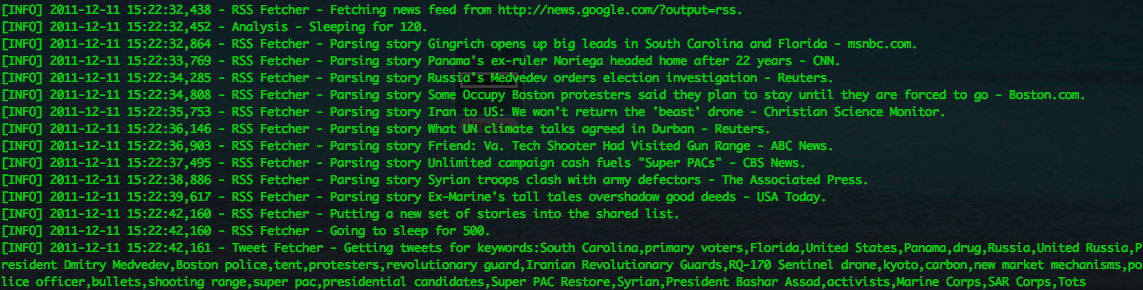
\includegraphics[scale=0.4]{logger.png}
				    \caption{Customised Logger}
	  \end{figure}
   \subsection{Unit and Mock Testing}

  	  We used the PyUnit\footnote{\url{http://pyunit.sourceforge.net/}} module for incorporating unit tests in our code. An example of where we used this was in the RSS thread where we were testing functionality of all the functions written for this module. For this we had to create a mock rss fetcher object and ran tests on it.
  	  
  	  Having said this, It was very difficult to test some parts of the system as there is a lack of clear models, for example having unit tests for keyword generation or tweet fetching is difficult to implement as they use external APIs.

		\subsection{UI Testing}
		To debug the UI, Google Chrome’s Developer tools and Firebug were used. These tools were used to inspect the requests the UI issued, the network activities, debug layout and monitor performance.
  
	\section{General Validation}
	
	\subsection{Keyword Relevancy}
  One of the most important part of the project was to find keywords for stories that would be specific enough to generate relevant tweets and general enough so that the amount of tweets we find is large enough to generate meaningful data. This proved to be troublesome and we had to constantly check if keywords look like they fit the data and monitor the amount of tweets matching each story and their quality. This was done manually, but if we were to continue developing the project an automatic monitoring tool would definitely have to be created.
	
		\subsection{User Validation}
  	  From time to time we asked for feedback on the user facing product, this was done so that we could make design and functionality choices. We talked to our supervisor Jeremy Bradley\footnote{\url{http://www.doc.ic.ac.uk/~jb}} and he liked our user interface but wanted us to add pictures for each news story, we consequently went ahead with this and received very positive feedback.
	
		\subsection{Code Validation}
		We used Pylint\footnote{\url{http://www.logilab.org/857}} to validate the python code which we wrote. This was done so that we could check if we had any bad indentation which could lead to silly errors. This also helped us check bad naming conventions for class names and functions.
	
		\subsection{UI Validation}
		http://validator.w3.org/ was used to validate the markup before pushing. We have a minimalist UI, therefore exhaustive tests were used to test all features.
	

		\subsection{Data Volume}

		Originally, there were problems with high write volumes, which was mostly due to improper use of writing debug information to files. This sometimes resulted in up to 30000 IO operations per second, resulting in emails from the VPS provider. This was subsequently solved, and IO volume is now proper.
	
		\begin{figure}[ht!]
					\centering
						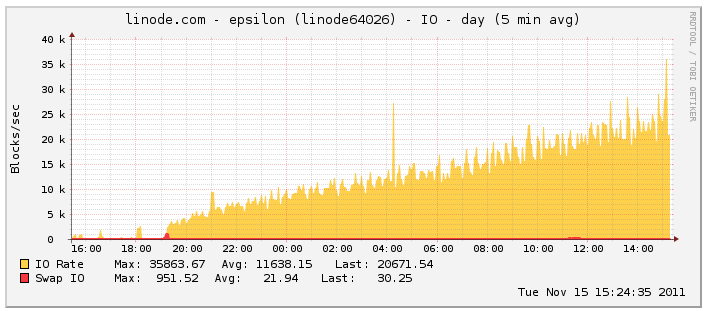
\includegraphics[scale=0.4]{io_chart.png}
					\caption{IO Volume before fix}
		\end{figure}
	
	
	\section{Managerial Documentation}
	
		\subsection{Collaboration Tools Used}
		
			\subsubsection{Git}
			
			We have used the git version control system for keeping track of the project, for easily reverting if there is a problem, and for having a very quick deploy mechanism. Whenever a code push occurs to our git repository, we have a git post-receive hook that copies the static files appropriately, and restarts the appropriate processes. This means that as soon as a code push occurs, the new version is live.
			
			\subsubsection{Trello}
			
			Trello\footnote{\url{http://trello.com}} is a very good piece of software by FogCreek. It is a digital board that allows you to create post-its and write the product backlog, and move tasks between the product backlog, the current iteration, and the finished tasks. We plan to extract and append the Trello history to our final report, to show progress. Here is a screenshot of how Trello works:
			
			\begin{figure}[ht!]
						\centering
							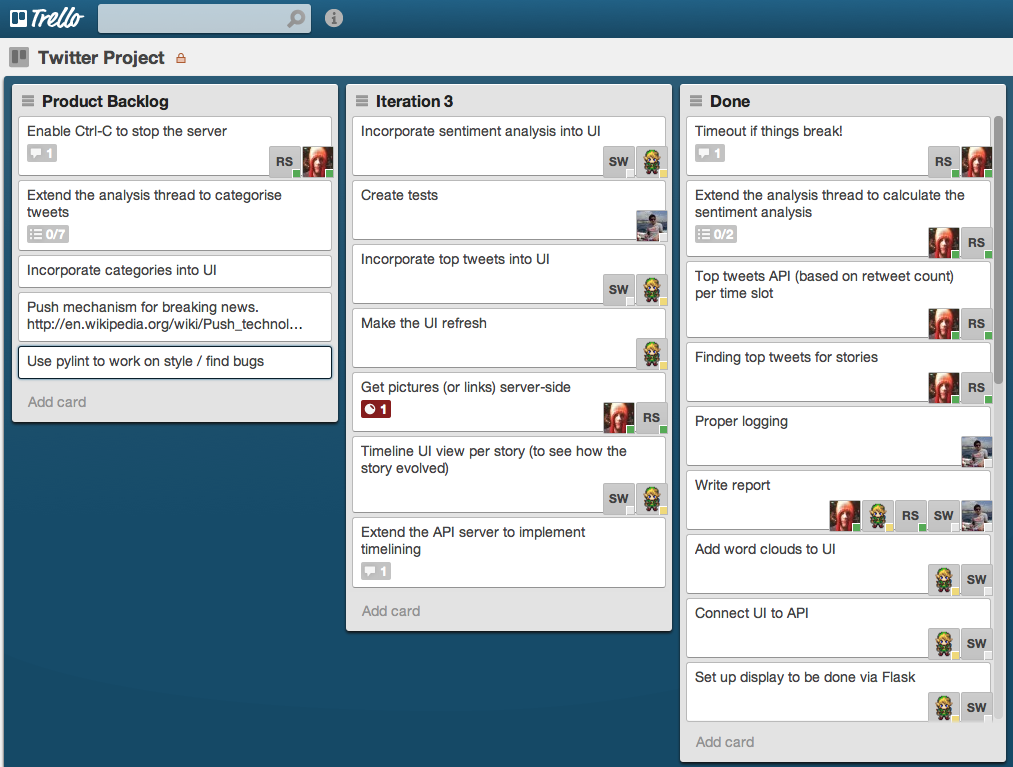
\includegraphics[scale=0.4]{trello1.png}
						\caption{Trello project management board}
			\end{figure}
			
			\subsubsection{Skype}
			
			We extensively used Skype to discuss the project and set up team meetings.
		
		\subsection{Management policies}
		
		Whenever a new code push occurs, it is immediately live on the server. We know that this is not particularly safe, as there is no server-side test suite that, if fails, prevents the new version from going live. Hence, we have asked all members to run the test suite locally, and see if the software works, before committing it to our main repository. This is definitely not ideal if our `live' environment was actually a production environment with real users depending on the code working, but we have decided that instead of over-burdening ourselves with extensive test suites and commit rules, we would concentrate more on adding user-visible features.
		
		\subsection{Management of knowledge transfer within the group}
		
		Knowledge transfer within the group was a non-issue, as we had worked with each other on another project. We were able to easily communicate all required information between group members even if not during a team meeting - be it over Skype, lunch, or in between lectures.
		
		On a number of occasions, just like planned in the initial report, we have used pair programming in the server-side team so that we were on the same page. This has worked well to distribute information, and inform the other people of what was done, and how it works, if they don't know. 
		
		We have planned for there to be more collaboration between the UI and the server side team, but unfortunately that didn't happen as much as we had wanted, and we have to say that the server side team does not actually know that much about the UI and how it works. Nevertheless, they have looked at it, and have a general idea of how it works if they were to continue or move teams to the UI. Part of the reason is probably that our project is very modular, and there was not much needed for the two teams to interact on the code-level.
	
	
  \subsection{Team Meetings}
  \begin{tabular}{c | l p{7cm} r}
    \emph{\large Date} &  \emph{\large Venue} &  \emph{\large Subject} &  \emph{\large Attended}\\
    \hline
    14/10/2011 & Lab Round Table & Choose which project to do & \(G\)\\
    18/10/2011 & Skypeland & Choose which project to do & \(G\)\\
    21/10/2011 & Lab Round Table & Discovered the original plan is infeasible due to constraints set by Twitter, draft backup plan & \(G\)\\
    27/10/2011 & Lab Round Table & Plan approved, Design Architecture & \(G \smallsetminus \{\texttt{Suhaib}\}\)\\
    3/11/2011 & Lab Round Table & Progress Report (Backend, and UI Prototype I) & \(G \smallsetminus \{\texttt{Rafal}\}\)\\
    10/11/2011 & Lab Round Table & UI Prototype II presentation, API requests and design & \(G \smallsetminus \{\texttt{Maciej}\}\)\\
    17/11/2011 & Lab Round Table & UI Prototype III. Post-JB-meeting discussion & \(G \smallsetminus \{\texttt{Jamal}\}\)\\
    24/11/2011 & Skypeland & Incremental improvements & \(G \smallsetminus \{\texttt{Sam}\}\)\\
    1/12/2011 & Skypeland & Extensions ideas & \(G \smallsetminus \{\texttt{Suhaib}\}\)\\
    8/12/2011 & Skypeland & Features prioritisation & \(G\)\\
  \end{tabular}
  \(G=\{\texttt{Rafal}, \texttt{Sam}, \texttt{Suhaib}, \texttt{Jamal}, \texttt{Maciek}\}\)\\
	
	\subsection{Member Contributions}
	  \subsubsection{Maciek Albin}
	    \begin{tabular}{l | p{10cm} r}
	     \emph{\large Date} & \emph{\large Comments} & \emph{\large Hours}\\
	     \hline
	     12/10/2011 & Advanced network generation for follower/folowee relations. & 3\\
	     20/10/2011 & More work on the network generation. & 4\\
	     28/10/2011 & Initial internal API definition and basic implementation. & 2\\
	     28/10/2011 & Fixes to inter thread communication. & 2\\
	     02/11/2011 & Refactoring. & 3\\
	     02/11/2011 & Implemented keyword generation using Alchemy API. & 2\\
	     03/11/2011 & Implemented basic analysis thread. & 4\\
	     04/11/2011 & Assigning tweets to stories in analysis thread. & 3\\
	     04/11/2011 & Added short summaries and links to stories DB. & 2\\
	     08/11/2011 & Added wordclouds to the API. & 1\\
	     10/11/2011 & Refactoring. & 3\\
	     30/11/2011 & Fixed bugs in the logger. & 2
	    \end{tabular}
	    
	  \subsubsection{Jamal Khan}
	  \begin{tabular}{l | p{10cm} r}
     \emph{\large Date} & \emph{\large Comments} & \emph{\large Hours}\\
     \hline
	  11/10/2011 & Initial creation of the RSS Fetcher using python module feedparser. & 2\\
    31/10/2011 & Keyword extraction completed for each story using Alchemy API. & 4\\
    4/11/2011 & Implemented Flask Server creating API for the front end for the site as well as relevant database calls to fetch stories. & 7\\
    10/11/2011 & Added functionality of getting stories by timestamp for the API. & 2\\
    25/11/2011 & Completed flexible logger for each thread, so we can see exactly what is going on. & 7\\
    12/11/2011 & Unit testing for RSS Fetcher completed. & 4
  \end{tabular}
  
  \subsubsection{Suhaib Sarmad}
    \begin{tabular}{l | p{10cm} r}
     \emph{\large Date} & \emph{\large Comments} & \emph{\large Hours}\\
     \hline
     27/10/2011 & Resource research and UI mockup & 4\\
     28/10/2011 & Basic grid UI proof of concept & 3\\
     09/11/2011 & Implementation of basic jQuery Masonry (tiled) UI & 2\\
     10/11/2011 & Create tiles in UI from server news API & 4\\
     11/11/2011 & CSS/HTML Tile layout, split into title/summary, picture, sentiment, word cloud, tweet list & 5\\
     11/11/2011 & UI debugging and cross-browser compatibility: works on all tested browsers except IE & 2\\
     12/11/2011 & Added tweets to tweet list using Twitter REST API and keywords from server API, added custom jQuery scrollbars & 1\\
     12/11/2011 & Added pictures to tiles using Google Images API and article titles & 2\\
     12/11/2011 & Generating html5 word cloud from keywords from server API & 3\\
     19/11/2011 & CSS3 transitions research and testing for big picture UI & 2\\
     01/12/2011 & Automatic refreshing and fetching of new news articles from server & 4\\
     09/12/2011 & Sentiment bar prototype & 1
    \end{tabular}
  
	
	  \subsubsection{Rafał Szymański}
	    \begin{tabular}{l | p{10cm} r}
	     \emph{\large Date} & \emph{\large Comments} & \emph{\large Hours}\\
	     \hline
	     10/10/2011 & Initial commit for the project. Basic implementation in Python of a script that given a keyword  fetches the live streaming API for the given keyword and writes it to the Mongo database. & 6\\
       11/10/2011 & Bug fixes and a short readme. & 2\\
       12/10/2011 & Fetching the follower/folowee graph and saving to a file. Basic analysis with NetworkX. & 3\\
       20/10/2011 & More working on generating the user graph. & 2\\
       21/10/2011 & Big update. Gets headlines from Google news RSS, generates keywords using Termtopia, sets up twitter stream, saves to Mongo and repeats every 5 minutes. & 7\\
       01/11/2011 & Improving the threading of the program - added condition variables and fixed previous threading bugs. & 4\\
       04/11/2011 & Working on instant deployment environment using Flask, Nginx, uwsgi, and a couple other technologies. Took forever to do but afterwards, after every git push, the new version is live straight away. & 10\\
       07/11/2011 & Improvements to the instant deployment - new git hook, and a control script that allows remote restarting and clearing of the database. & 4\\
       08/11/2011 & Wordcloud generation. Goes through each tweet, finds the most occurring words and adds that data for each analysis period. & 4\\
       11/11/2011 & Improvements to control script. & 2\\
       30/11/2011 & Sentiment analysis for each period. Gets sentiment using an API and adds to Mongo. & 5\\
       04/12/2011 & Top tweets based on the number of retweets. & 2\\
       04/12/2011 & Added all my new data to the frontend API. & 2
	    \end{tabular}
	  
	  \subsubsection{Sam Wong}
	  \begin{tabular}{l | p{10cm} r}
     \emph{\large Date} & \emph{\large Comments} & \emph{\large Hours}\\
     \hline
	   12/10/2011 & Python development & 1\\
     02/11/2011 & UI Prototype 1 & 3\\
     09/11/2011 & UI Prototype 2 & 4\\
     20/11/2011 & UI Prototype 3 & 5\\
     21/11/2011 & UI debugging & 1\\
     25/11/2011 & UI features experimentation & 1\\
     01/12/2011 & UI features refinement & 1\\
     01/12/2011 & Auto-refresh & 2\\
     01/12/2011 & infinite scroll proof of concept & 3\\
    \end{tabular}

		\section{Overview}
		
		\subsection{Usage of Scrum}
		
		In the two previous projects, and after having read a lot about Agile and Scrum development methodologies, we were very excited to use these techniques, and have set up plans for that, but such scrum meetings mostly didn't happen. Scrums are very frequent meetings, which means that everyone has to actually have done something the day before - this wasn't the case in our project.
		
		The problem is that scrum is more geared towards full-time developers who produce code every day, and in our project, there were periods where we haven't done anything for a week due to coursework, studying, or other preoccupations. Hence, instead of having scrum meetings, we mostly just discussed the project in between lectures and in labs. We realize that scrum is probably a good choice, but only in situations where everyone is a full time developer and has the time to contribute code every day.
  

\end{document}
